%% ============================================================
% f2012_sichuan_sci_q19_pyramid.tex
%% 2012 四川卷（理科）第 19 题 三棱锥 P-ABC，∠APB=90°，∠PAB=60°，平面PAB⊥平面ABC
%% 来源 PDF：普通高考/2012/2012四川理.pdf 第 2 页（印面 772）第 1 栏
%% 坐标取自原页矢量层（bp），原点为图区左上角 (230.0,525.0)，y 向下；虚线照原页。
%% ============================================================
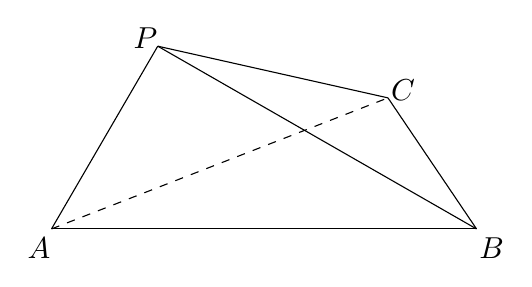
\begin{tikzpicture}[x=1bp,y=-1bp,
  every node/.style={inner sep=0,font=\fontsize{10.5pt}{12.6pt}\selectfont},
  line cap=butt, line join=miter]
  \draw[line width=0.3985bp] (8.547,74.539) -- (161.559,74.539);
  \draw[line width=0.3985bp] (161.559,74.539) -- (129.68,27.359);
  \draw[line width=0.3985bp] (129.68,27.359) -- (46.801,8.746);
  \draw[line width=0.3985bp] (46.801,8.746) -- (8.547,74.539);
  \draw[line width=0.3985bp] (46.801,8.746) -- (161.559,74.539);
  \draw[line width=0.3985bp, dash pattern=on 2.989bp off 2.989bp] (8.547,74.539) -- (129.68,27.359);
  \node[anchor=base west] at (37.87,9.54) {$P$};
  \node[anchor=base west] at (130.62,28.16) {$C$};
  \node[anchor=base west] at (-0.23,85.22) {$A$};
  \node[anchor=base west] at (162.39,85.22) {$B$};
\end{tikzpicture}
